\graphicspath{{content/chapters/5_design/figures/}}
\chapter{Desing}
\label{chp:design}

\section{Project Structure}
\label{sec:project_structure}

The overall structure of the project is modular, enabling clean separation of concerns and supporting future extensibility. The project is organized around three main pipelines: \textbf{training}, \textbf{denoising}, and \textbf{deployment}. Each pipeline is implemented as a collection of dedicated modules, coordinated through the central \texttt{main.py} script, which serves as the entry point for running the system.

The training and denoising pipelines constitute the core of the project and are discussed in detail throughout this report. The deployment pipeline is discussed separately in Chapter~\ref{chp:deployment}, following the evaluation of model performance.

To maintain clarity and modularity, all helper modules are organized within a \textit{Utils} directory. This directory contains the core functionality for dataset handling, model definitions, training routines, inference logic, and baseline methods. Additionally, a centralized configuration file, \texttt{config.py}, located alongside \texttt{main.py}, manages all project parameters using a dictionary-based structure. This design allows users to easily modify hyperparameters or experiment settings in a single location, improving usability and reproducibility.

An overview of the key files in the \textit{Utils} directory is provided below:

\begin{itemize}
    \item \texttt{dataset.py}: Contains all dataset classes used in the project, implemented as PyTorch \texttt{Dataset} objects. The file supports multiple strategies for handling variable-length audio inputs, as discussed in Section~\ref{sec:variable_length_handling}. It also defines the \texttt{BucketSampler} class for length-based batch sampling, the \texttt{pto\_collate} function for efficient collation, and a visualization utility for analyzing padding distribution.

    \item \texttt{model.py}: Defines the neural network architectures used for speech enhancement. Each model is implemented as a subclass of PyTorch’s \texttt{nn.Module}, and the module is designed for easy experimentation with new architectures or changes in hyperparameters.

    \item \texttt{train.py}: Implements the training loop, validation logic, and performance tracking. It supports training using any of the dataset classes defined in \texttt{dataset.py}, allowing for flexible experimentation with different data-handling strategies.

    \item \texttt{denoise.py}: Handles inference and evaluation post-training. It mirrors the training pipeline structure but focuses on running the model in inference mode and computing objective metrics. The module also allows switching between learned models and classical methods for direct comparison.

    \item \texttt{classical.py}: Implements traditional signal processing–based denoising algorithms used as baseline comparisons. These functions operate on waveform inputs and are implemented using either custom code or well-established signal processing libraries where appropriate.
\end{itemize}

\section{Variable Length Handling}
\label{sec:variable_length_handling}

For this project, only the clean and noisy pairs of audio files from the dataset are required — the transcript text files are ignored, as they are not relevant to the task. However, it is worth noting that such transcripts are highly valuable in other applications, such as training text-to-speech or speech recognition models. As highlighted in the dataset analysis in Section~\ref{sec:dataset_exploration}, the audio files vary in length. This poses a challenge for model training, as batch processing requires input tensors to have consistent dimensions.

To address this, several algorithms for handling variable-length audio inputs were explored. The most basic approach involves padding each audio file to match the length of the longest sample in the batch, typically by appending zeros to the end of shorter files. While this method is simple, it has significant drawbacks: excessive padding introduces unnecessary data that may act as noise during training, making it harder for the model to learn effectively. The greater the variation in input lengths, the more padding is required — which can negatively impact overall training performance.

\begin{figure}[h]
    \centering
    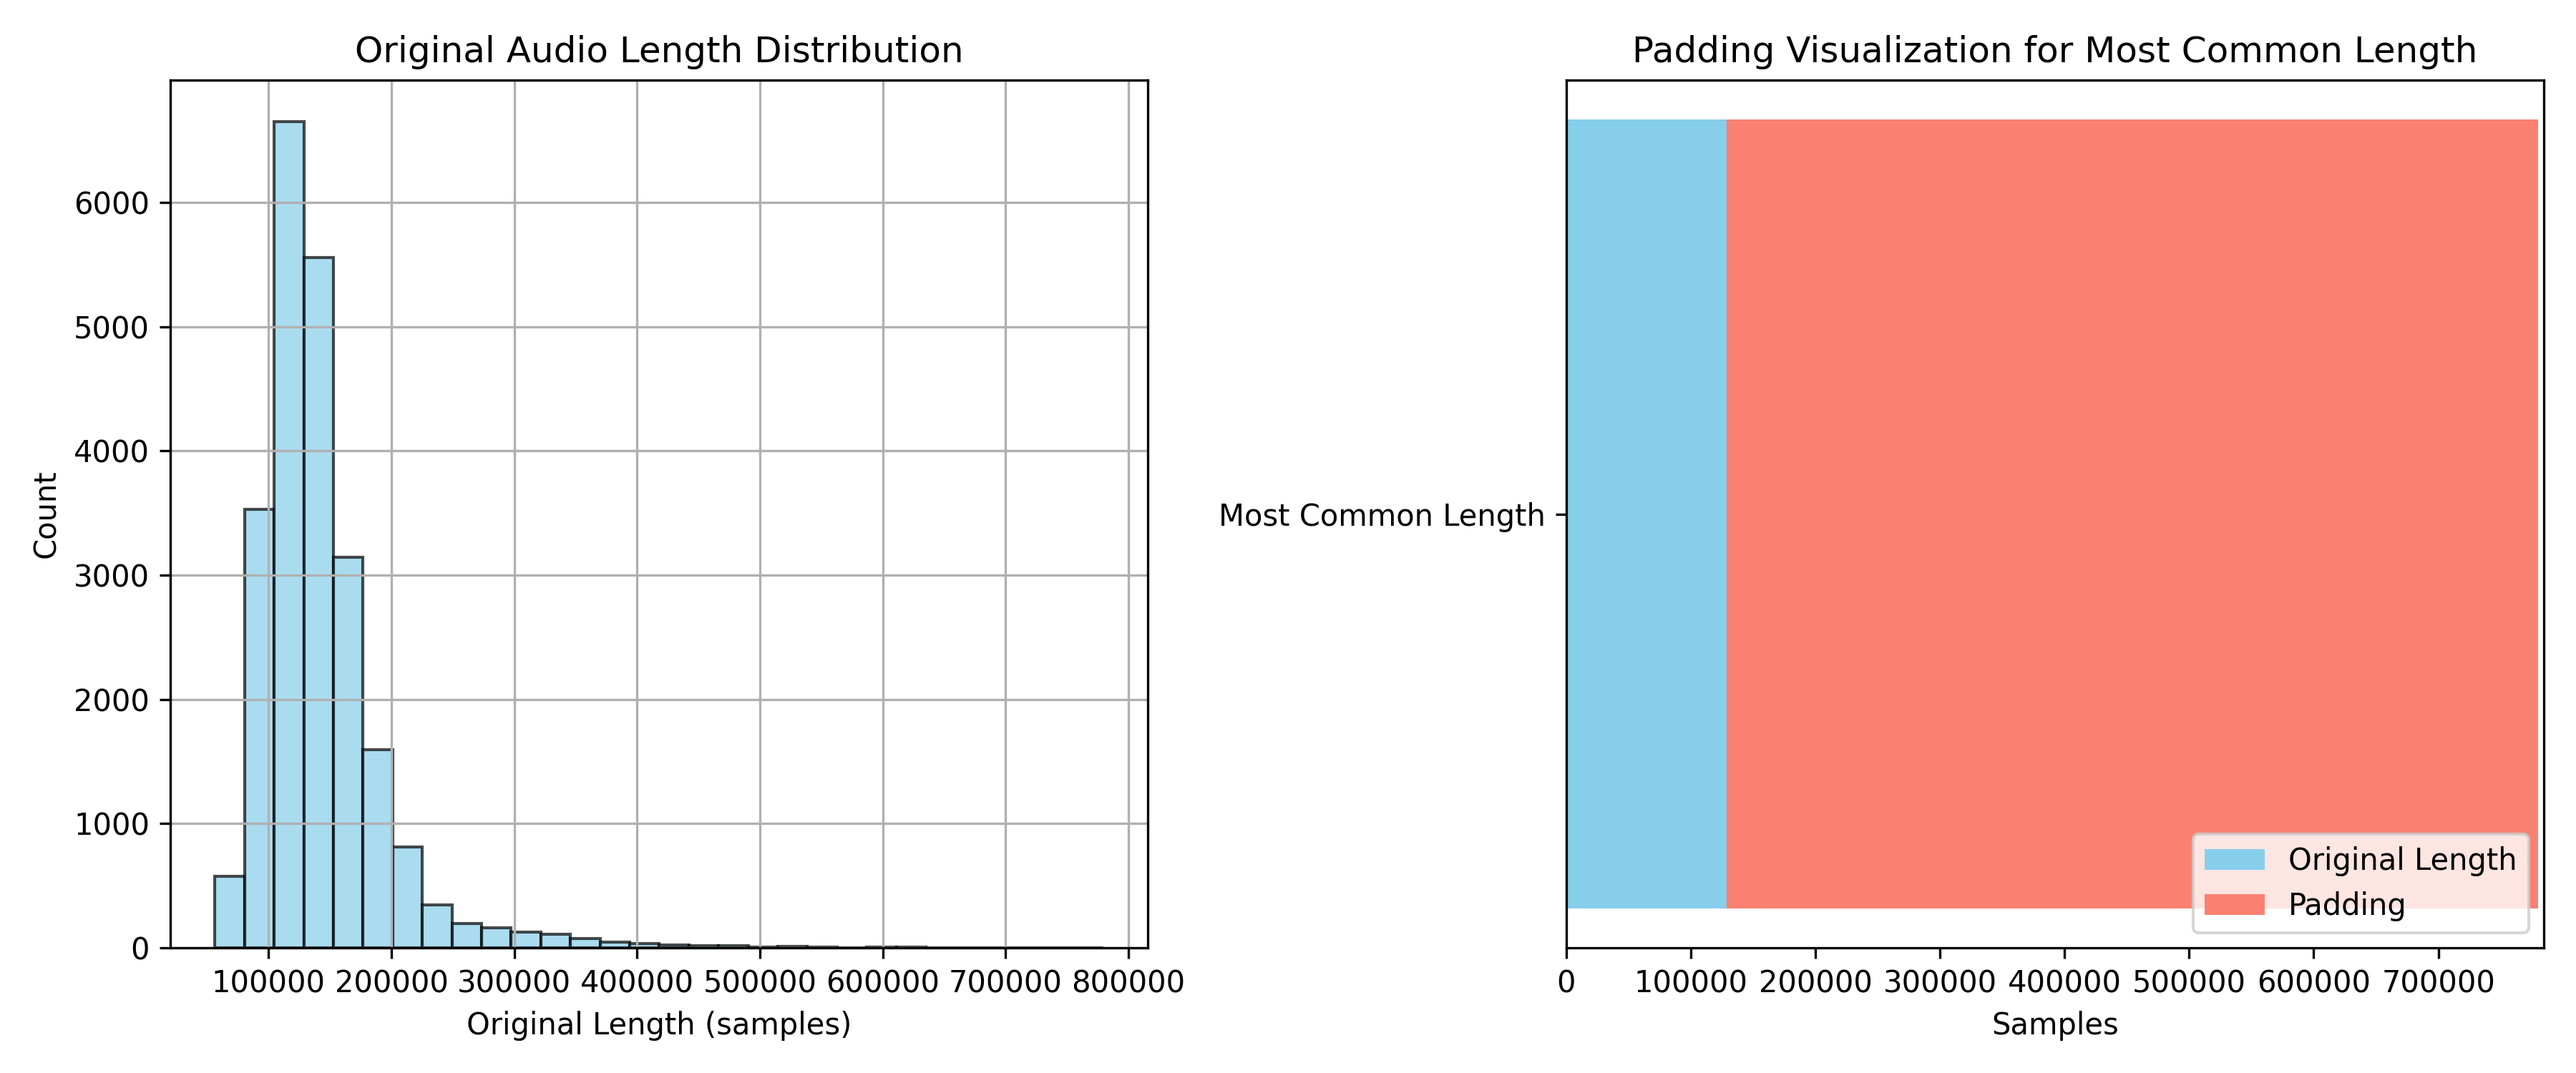
\includegraphics[width=\textwidth,keepaspectratio]{max_padding.png}
    \caption{\label{fig:max_padding}Illustration of maximum-length padding.}
\end{figure}

As shown in Figure~\ref{fig:max_padding}, the most common audio length is padded so heavily that the padding exceeds the actual content. This is far from ideal. To mitigate this issue, three different padding strategies were implemented. Each method aims to reduce the impact of excessive padding on model performance.

The first method is \textit{Static Bucketing}, which groups audio files into predefined fixed-length buckets. Building on this, the second method, \textit{Dynamic Bucketing}, creates buckets dynamically based on the distribution of audio lengths, offering a more adaptive grouping approach. The third and final method, inspired by a research paper~\cite{yoon2020pto}, proposes a simple, distortion-free technique for handling variable-length sequences through a combination of padding, truncation, and output truncation.

All three methods were implemented for testing and evaluation. Their role in the system design is critical, as they help ensure that the model can learn effectively without being hindered by dimensional mismatches or excessive zero-padding. Further details on the implementation of these methods are provided in Chapter~\ref{chp:implementation}, and their impact on model performance is discussed in Chapter~\ref{chp:evaluation}.

\section{Model Architecture}
\label{sec:model_architecture}

The model architecture is the highlight of the system design. It is the core component that determines how the system processes input data, how hidden layers and their connections are defined, and how the final output is generated. The modular design of the project as a whole facilitates the exploration of various model architectures. The main structure for speech enhancement models has already been introduced in Chapter~\ref{chp:literature_review}. With the concept of autoencoders being well-established in the literature, the most basic model defined in this work is a convolutional neural network (CNN) autoencoder.

\subsection{Convolutional Neural Network (CNN)}

The CNN model implemented in this project serves as the baseline architecture. It is designed as a basic encoder-decoder model that operates directly on the real and imaginary components of the spectrogram, which are concatenated into a two-channel input. The encoder compresses the input using a series of three simple convolutional blocks, each consisting of a convolutional layer followed by a PReLU activation function. The encoder progressively reduces the spatial dimensions while increasing the depth of the feature maps, allowing the model to learn increasingly abstract representations of the input data.

\begin{figure}[h]
    \centering
    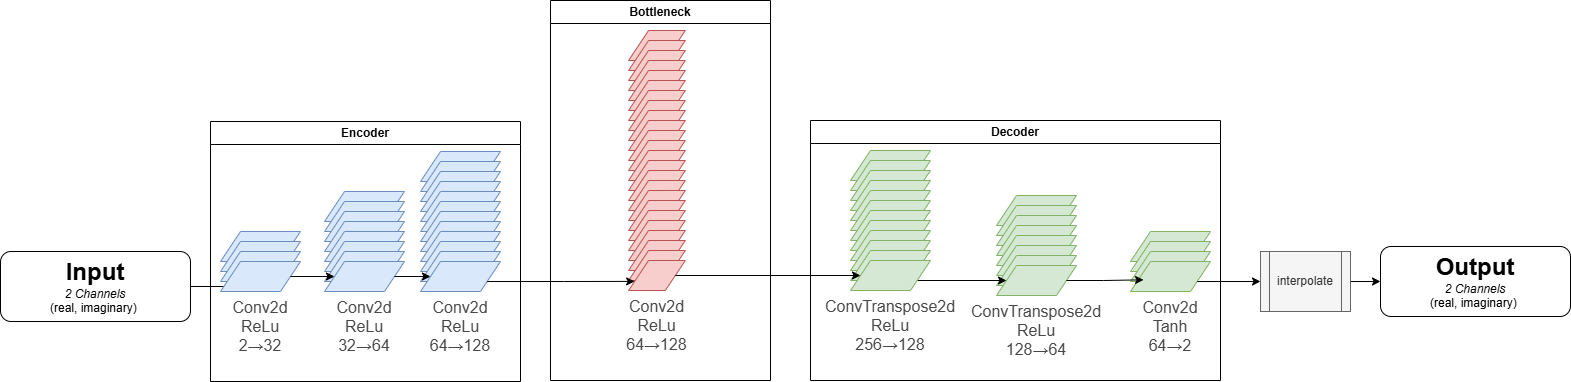
\includegraphics[width=\textwidth,keepaspectratio]{cnn.png}
    \caption{\label{fig:cnn}Basic CNN architecture.}
\end{figure}

The encoder then passes the compressed representation to the bottleneck layer, which is used to further transform the feature space and encourage the model to learn a more compact and expressive representation of the input. Bottleneck layers in deep learning architectures are often used to reduce the dimensionality of the latent representation, act as a regularizer, or increase non-linearity before reconstruction. In this implementation, the bottleneck is intentionally kept simple: it consists of a single additional convolutional layer with a higher channel depth (126 -> 256), followed by a PReLU activation function. This layer is placed outside of the encoder and decoder blocks to preserve architectural modularity and to isolate the representation-learning stage from the downsampling and upsampling operations. While not a traditional bottleneck in terms of dimensionality reduction, it acts as a feature transformer and deepens the network's capacity without affecting the input/output resolution.

Following the bottleneck, the decoder reconstructs the spectrogram from the transformed latent features. It mirrors the encoder structure by using two transposed convolutional layers (also known as deconvolution layers), each followed by a PReLU activation function. These layers progressively upsample the feature maps, restoring the spatial dimensions that were reduced during the encoding process. The decoder is responsible for reintroducing fine-grained details and structural patterns necessary to reconstruct a clean version of the original spectrogram from its compressed representation.

The final layer of the network is a standard convolutional layer that reduces the number of channels from 64 to 2, corresponding to the real and imaginary parts of the denoised spectrogram. This layer is followed by a \texttt{Tanh} activation function, which constrains the output values to the range \([-1, 1]\), making the output suitable for reconstruction and audio playback. This range is especially useful when reconstructing signals that will later be passed through an inverse Short-Time Fourier Transform (iSTFT), where stability and boundedness are beneficial.

While simple, this model plays a critical role in establishing a baseline performance level. It ensures that the overall system functions correctly while providing a reference point for evaluating the impact of architectural modifications. The CNN model is straightforward to implement and interpret, making it a suitable starting point for benchmarking and for guiding the development of more sophisticated architectures introduced in subsequent sections.

\subsection{Convolutional Encoder Decoder (CED)}

The Convolutional Encoder Decoder (CED) architecture implemented in this project is based on the model proposed by Park and Lee (2017) \cite{park2017acoustic}. It is specifically designed for the task of speech enhancement and operates directly on spectrogram data. The CED model follows a symmetric encoder-decoder structure without an explicit bottleneck, and is optimized for temporal feature extraction using frequency-preserving convolutional kernels. The real and imaginary components of the spectrogram are concatenated to form a two-channel input, consistent with the input formatting of the baseline CNN.

\begin{figure}[h]
    \centering
    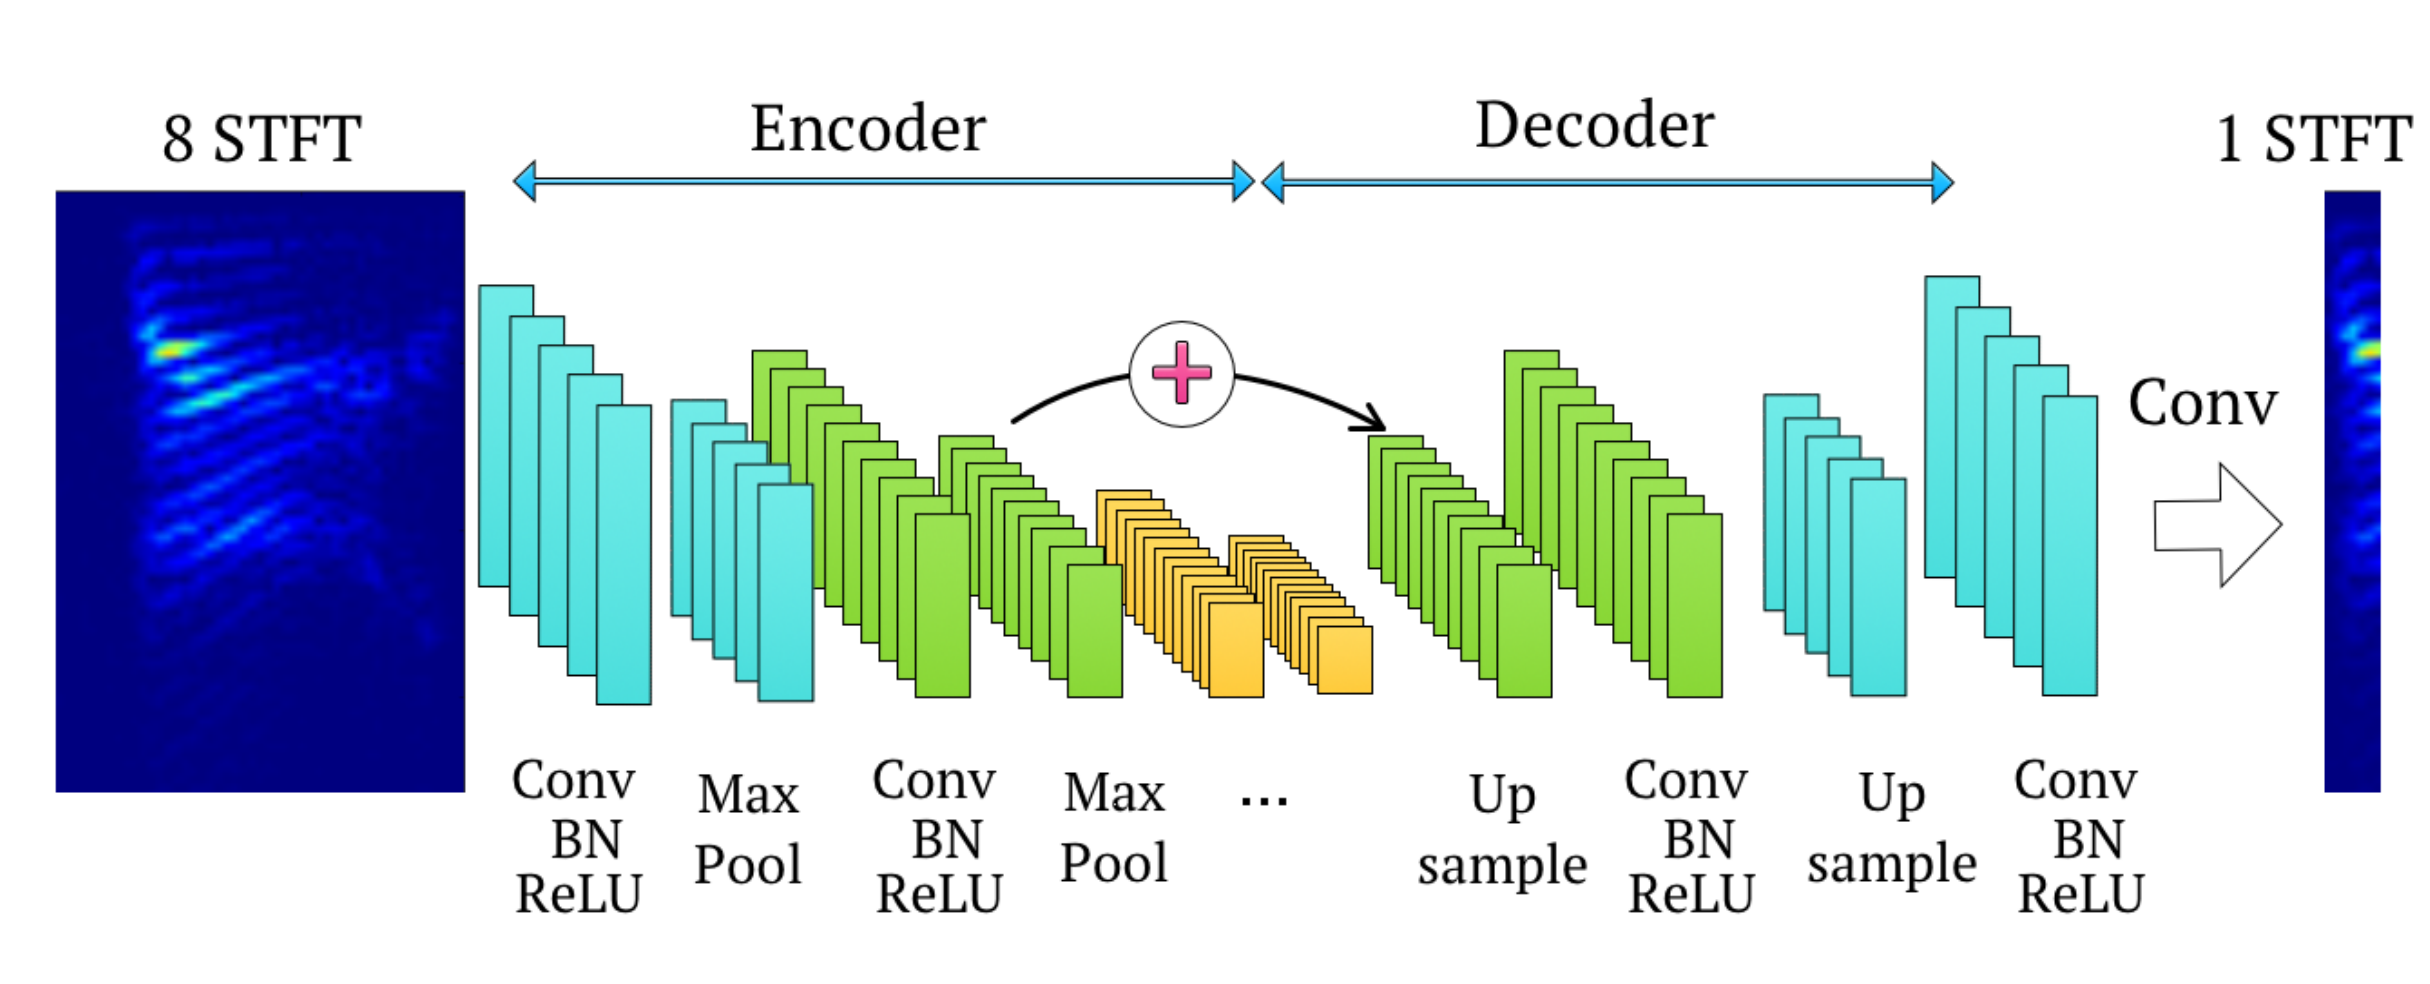
\includegraphics[width=\textwidth,keepaspectratio]{ced.png}
    \caption{\label{fig:ced}Convolutional Encoder Decoder (CED) Network\cite{park2017acoustic}.}
\end{figure}

The encoder is composed of five convolutional blocks. Each block consists of a convolutional layer with a tall vertical kernel (ranging from \(13 \times 1\) to \(5 \times 1\)), followed by batch normalization, a ReLU activation function, and a \(2 \times 1\) max pooling operation. These blocks progressively downsample the temporal resolution while preserving frequency content, allowing the model to focus on temporal patterns critical for speech structure. As the signal propagates through the encoder, the number of feature channels increases (from 12 up to 32), allowing for richer and more abstract representations to be learned.

In contrast to the baseline CNN, the CED model omits a distinct bottleneck layer. Instead, the compressed representation at the output of the encoder directly feeds into the decoder. The decoder mirrors the encoder using upsampling layers followed by convolution, batch normalization, and ReLU activation. This upsampling progressively restores the temporal resolution of the feature maps to match the original input shape.

A final convolutional layer with a large vertical kernel size of \(129 \times 1\) is used to project the decoder’s output to two channels corresponding to the real and imaginary components of the enhanced spectrogram. This layer is followed by a \texttt{Tanh} activation function to ensure the outputs are bounded within the range \([-1, 1]\), which is beneficial for numerical stability during inverse transformations such as the iSTFT.

By removing the bottleneck and relying on deeper convolutional transformations, the CED model allows for a smoother flow of information from input to output. Its symmetric structure and tailored kernel dimensions make it particularly well-suited for speech enhancement, as demonstrated in the original work by Park and Lee. In this project, the CED serves as a strong benchmark to evaluate the benefits of deeper temporal modeling compared to the simpler CNN baseline.

\subsection{Redundant Convolutional Encoder Decoder (R-CED)}

The Redundant Convolutional Encoder Decoder (R-CED) architecture implemented in this project is directly adapted from the model proposed by Park and Lee (2017) \cite{park2017acoustic}. It is a fully convolutional architecture developed as a modification to the CED framework, specifically designed to eliminate the need for pooling and upsampling layers. This design prioritizes maintaining temporal and frequency resolution throughout the network, addressing the potential drawbacks of information loss associated with aggressive downsampling in traditional encoder-decoder structures.

\begin{figure}[h]
    \centering
    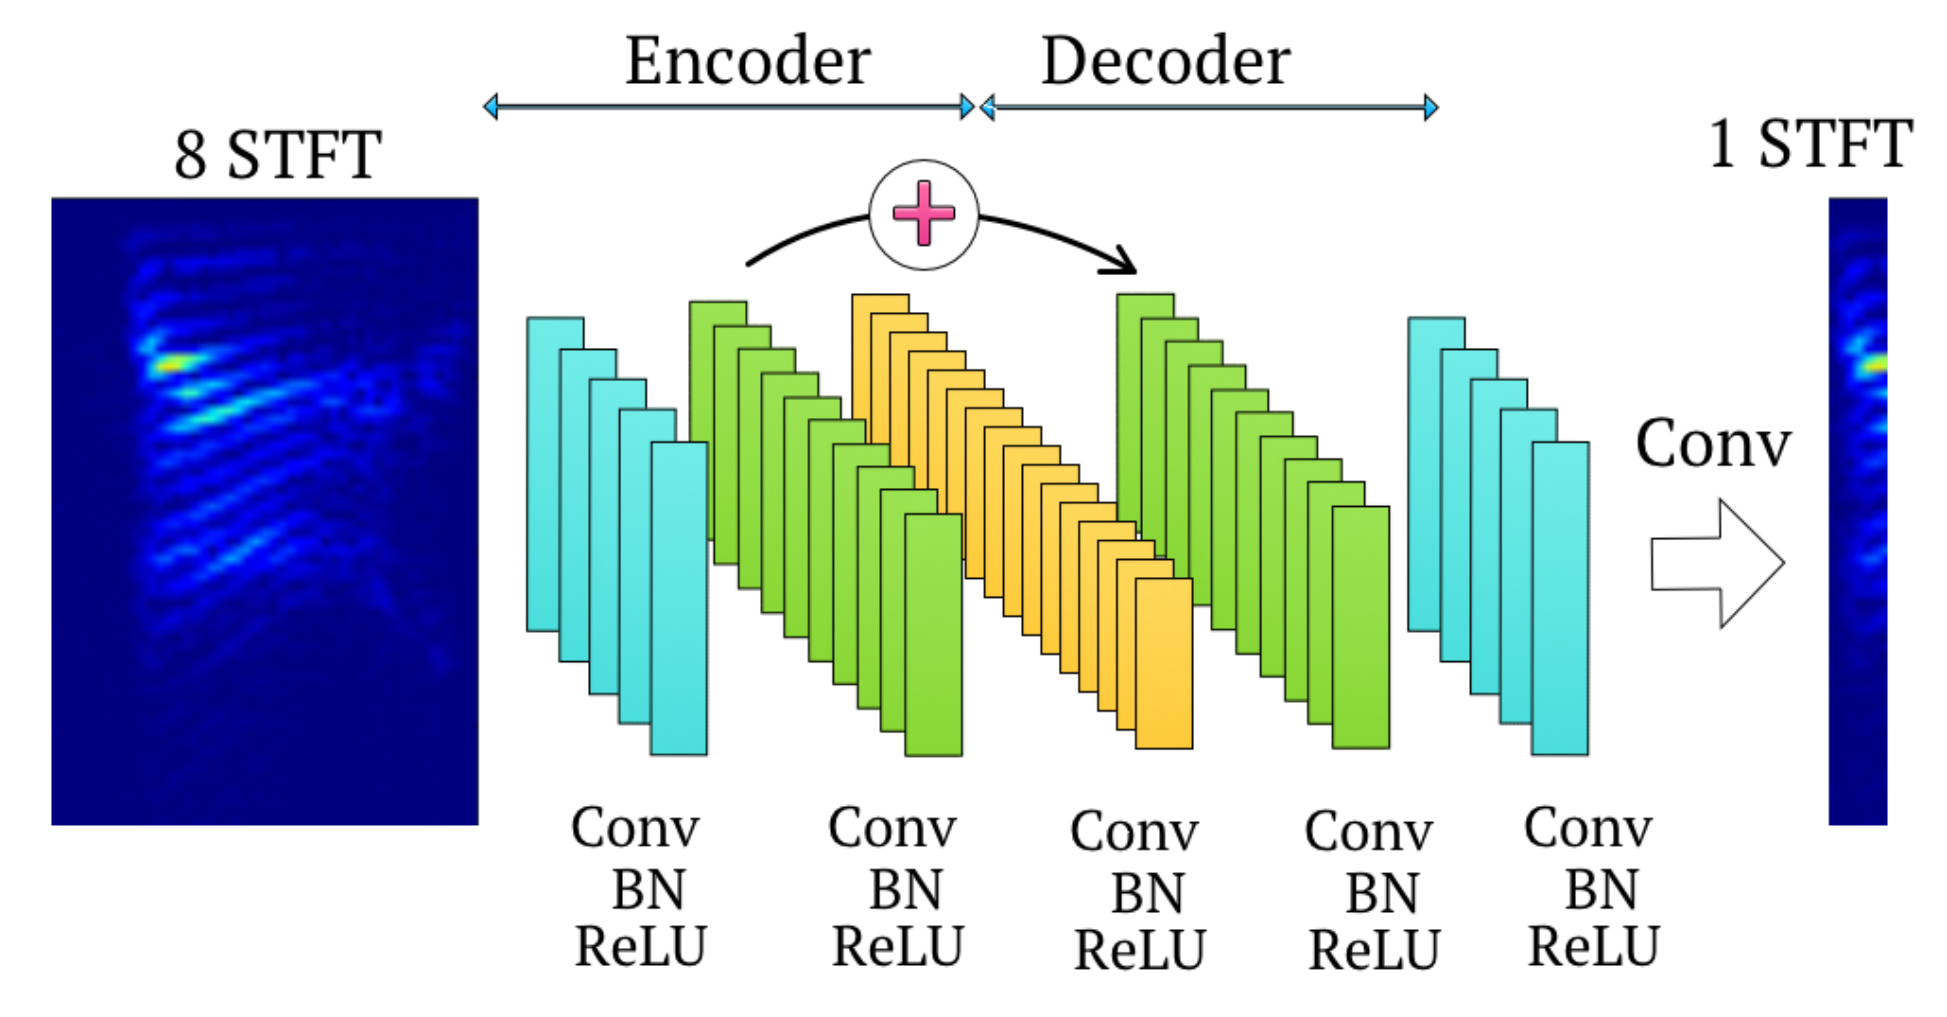
\includegraphics[width=\textwidth,keepaspectratio]{r-ced.png}
    \caption{\label{fig:rced}Redundant Convolutional Encoder Decoder (R-CED) architecture \cite{park2017acoustic}.}
\end{figure}

The R-CED architecture comprises a series of convolutional layers applied in sequence, with no intermediate pooling or upsampling operations. Each convolutional block consists of a vertically oriented convolutional layer (e.g., \(13 \times 1\), \(11 \times 1\), etc.), followed by a ReLU activation and batch normalization. These layers are stacked symmetrically around the center of the network, forming a deep pipeline of transformations that preserve the input's resolution at each stage.

The key innovation in the R-CED model is the use of **redundant convolutional layers** — that is, multiple layers with matching input and output dimensions — which serve to increase the network’s capacity without reducing the temporal fidelity of the signal. According to the authors, this redundant structure helps the model learn more complex transformations over the same resolution domain, enabling superior denoising performance without sacrificing the granularity of spectrogram features.

At the end of the network, a final convolutional layer with a large vertical kernel (\(129 \times 1\)) projects the output to two channels representing the denoised real and imaginary spectrogram components. As in the CED architecture, a \texttt{Tanh} activation is applied to bound the output within \([-1, 1]\), which facilitates stable reconstruction when applying the inverse STFT.

In contrast to both the baseline CNN and the CED model, the R-CED does not compress or expand the temporal resolution of the data. Instead, it relies entirely on the expressive capacity of multiple convolutional layers to model the mapping from noisy to clean spectrogram representations. This makes R-CED particularly suitable for applications where retaining precise time-frequency alignment is critical. In this project, the R-CED model is evaluated as a lightweight yet expressive alternative to deeper encoder-decoder variants.

\subsection{U-Net}

The U-Net model implemented in this project is adapted from the well-established U-Net architecture originally developed for biomedical image segmentation. In this work, the model is repurposed for complex spectrogram enhancement. It processes the real and imaginary components of the STFT spectrogram as a two-channel input and learns to generate a denoised spectrogram through a fully convolutional encoder-decoder structure with skip connections \cite{ronneberger2015unet}.

The core structure of U-Net is symmetric, comprising five downsampling stages (encoder), a bottleneck layer, and five upsampling stages (decoder). Each encoder block consists of a convolutional layer followed by instance normalization and a PReLU activation. Instance normalization is chosen over batch normalization to provide improved memory efficiency and stability when dealing with variable-length or low-batch-size audio inputs. The encoder progressively compresses the spatial resolution of the input while increasing the number of feature channels, allowing the network to capture increasingly abstract spectral patterns.

\begin{figure}[h]
    \centering
    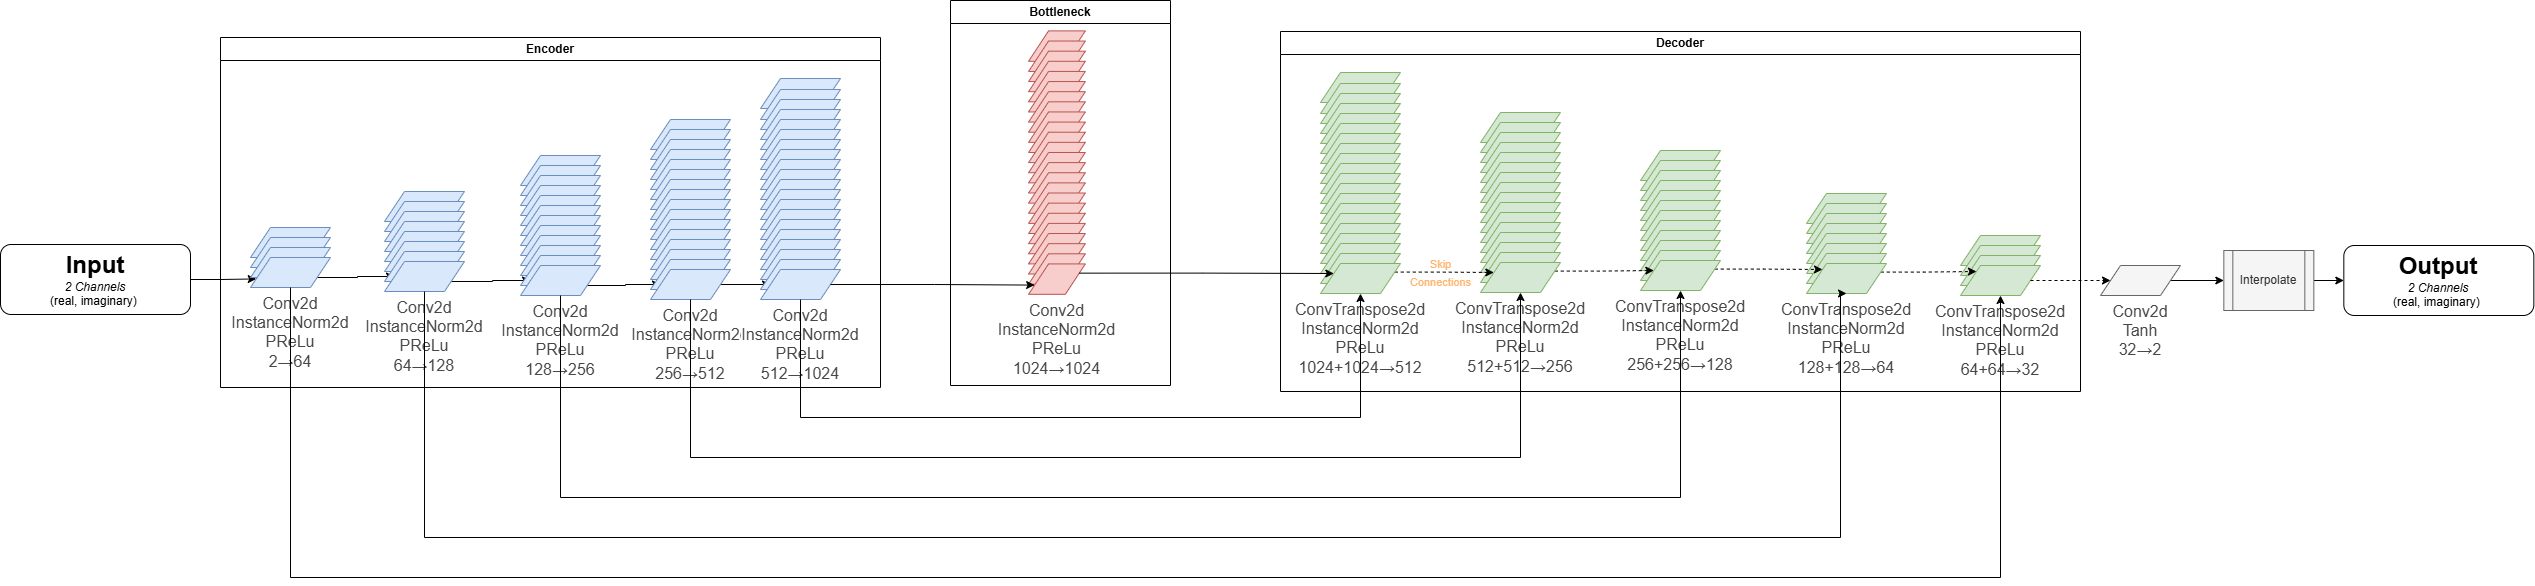
\includegraphics[width=\textwidth]{unet.png}
    \caption{\label{fig:unet}U-Net architecture used for complex spectrogram enhancement.}
\end{figure}

The encoder consists of five convolutional blocks. The first block receives the two-channel input (real and imaginary) and outputs 64 feature maps. Each subsequent block doubles the number of channels (from 64 to 128, 256, 512, and finally 1024), while applying a stride of 2 to downsample the feature maps in the time dimension. At the end of the encoder, the final feature map of size 1024 channels is passed into the bottleneck.

The bottleneck acts as the central transformation layer in the model. It comprises a single convolutional block with 1024 input and output channels, preserving the depth of the latent representation while providing non-linear transformation capabilities. Unlike traditional bottleneck layers that reduce dimensionality, this layer serves as a deep transformation point prior to decoding, facilitating high-capacity feature extraction.

The decoder mirrors the encoder structure with five upsampling blocks. Each decoder block performs a transposed convolution to upsample the feature maps and reduce the number of channels. Additionally, each decoder stage receives a skip connection from the corresponding encoder block. These skip connections concatenate feature maps from the encoder to the decoder at the same hierarchical level, providing direct access to low-level details that may otherwise be lost during downsampling. The concatenated feature maps are then processed by the transposed convolution layers, followed by instance normalization and PReLU activation. This skip connection mechanism greatly enhances the model’s ability to preserve fine-grained spectro-temporal structures in the output.

The final decoder block reduces the feature maps to 32 channels. This is followed by a standard $3 \times 3$ convolutional layer that projects the output to two channels, corresponding to the real and imaginary components of the denoised spectrogram. A $\tanh$ activation is applied at the output to constrain the values within the range \([-1, 1]\), ensuring stable reconstruction and alignment with the expected value range for audio waveforms. Lastly, a bilinear interpolation step ensures the output size matches the input spectrogram, compensating for any rounding errors introduced during downsampling and upsampling.

This implementation of U-Net preserves the key architectural principles of the original model while tailoring it for speech enhancement. The use of instance normalization, PReLU activations, skip connections, and a deeper encoder-decoder path provides the network with strong representational power, allowing it to effectively recover clean speech from noisy spectrograms.

\subsection{Convolutional Time-domain Audio Separation Network (Conv-TasNet)}

Conv-TasNet is a convolutional neural network architecture originally proposed by Luo and Mesgarani in their 2019 paper, \textit{``Conv-TasNet: Surpassing Ideal Time--Frequency Masking for Speech Separation''} \cite{luo2019conv}. The model was designed to operate directly on raw waveform inputs in the time domain, demonstrating superior performance to traditional time--frequency masking methods. The architecture consists of three main components: an encoder, a temporal convolutional network (TCN) for separation, and a decoder, as visualized in Figure~\ref{fig:convtasnet}.

\begin{figure}[h]
    \centering
    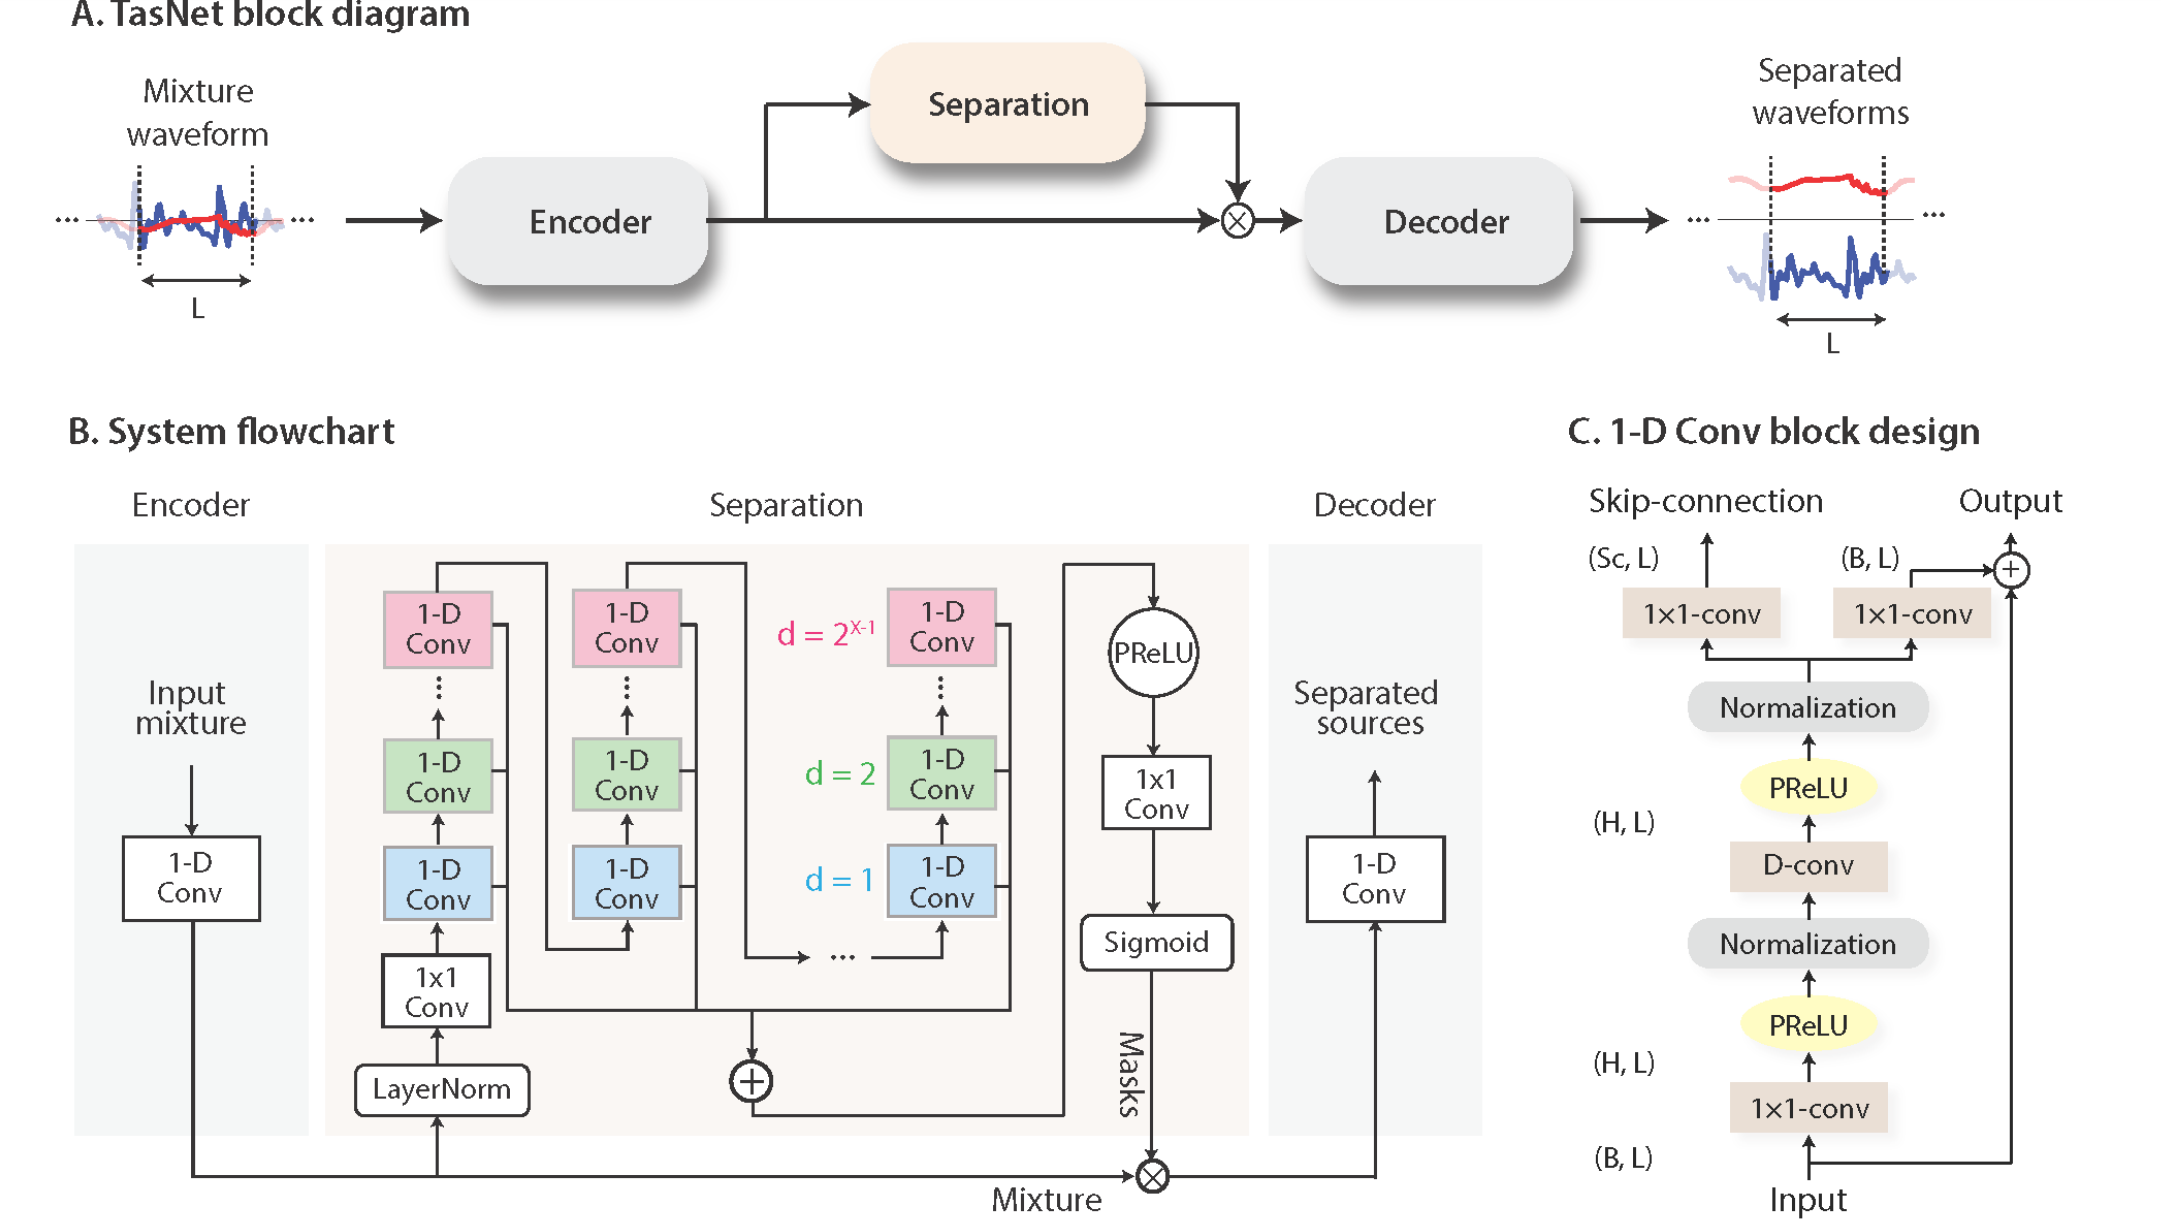
\includegraphics[width=\textwidth,keepaspectratio]{conv-tasnet.png}
    \caption{\label{fig:convtasnet}Conv-TasNet architecture overview \cite{luo2019conv}.}
\end{figure}

The \textbf{encoder} transforms the input mixture waveform into a latent representation using a 1D convolutional layer. This encoded representation is then passed to the \textbf{separation module}, which consists of multiple stacked convolutional blocks organized as a Temporal Convolutional Network (TCN). Each TCN block contains dilated depthwise separable convolutions, layer normalization, and PReLU activations. A residual connection ensures effective gradient propagation and allows the network to model long-range temporal dependencies efficiently. The separation module estimates masks for each speaker or clean component, which are applied to the encoded features.

The \textbf{decoder} reconstructs the clean waveform from the masked latent representation using a transposed 1D convolution layer, mirroring the encoder’s structure. This design enables end-to-end optimization without relying on time--frequency representations such as the STFT.

\subsubsection*{Adaptation for This Project}

While the original Conv-TasNet operates entirely in the time domain, the implementation in this project adapts the architecture for \textit{complex-valued spectrogram input}, which is more suited to denoising tasks in spectral space. Instead of raw audio, the model receives the real and imaginary parts of the spectrogram as separate input channels. The encoder and decoder are implemented using 2D convolutions to handle the frequency-time structure of the spectrogram. The TCN separation module preserves the core ideas of stacked dilated residual blocks with skip connections but is adapted for 2D convolutional processing.

This approach enables the model to benefit from Conv-TasNet’s efficient and powerful separation mechanism while remaining compatible with the spectrogram-based processing pipeline used throughout this project.


\subsection*{Summary}

The development of the model architectures in this project reflects a systematic exploration of both foundational and state-of-the-art neural network designs for speech enhancement. Starting from a simple CNN-based autoencoder, which establishes a reliable and interpretable baseline, the project progresses to more sophisticated architectures including the Convolutional Encoder Decoder (CED) and Redundant CED (R-CED), both of which are based on established research in speech enhancement literature \cite{park2017acoustic}. These architectures introduce structural innovations such as deeper convolutional hierarchies and redundancy without resolution loss.

Building upon this, the U-Net architecture leverages skip connections and a deep encoder-decoder pathway to improve information flow and detail preservation across layers. Finally, the project incorporates an adaptation of the Conv-TasNet model \cite{luo2019conv}, a powerful TCN-based architecture originally designed for end-to-end speech separation, repurposed here to operate on complex-valued spectrograms for denoising tasks.

By designing and implementing this diverse set of models, the project aim to provide a robust comparison of learning-based techniques, evaluate their architectural trade-offs, and ultimately benchmark them against classical signal processing approaches.



